\documentclass[aspectratio=169,11pt]{beamer}

% =========================================================
% MADRID + SQUARE GRID PhD PRESENTATION TEMPLATE
% =========================================================

% ---------------------------------------------------------
% THEME
% ---------------------------------------------------------
\usetheme{Madrid}

% ---------------------------------------------------------
% PACKAGES
% ---------------------------------------------------------
\usepackage[T1]{fontenc}
\usepackage{lmodern}
\usepackage{amsmath}
\usepackage{amssymb}
\usepackage{booktabs}
\usepackage{tikz}

\usetikzlibrary{
	positioning,
	arrows.meta,
	shapes.geometric,
	calc
}

% ---------------------------------------------------------
% COLOURS
% ---------------------------------------------------------
\definecolor{CyberBlue}{RGB}{25,85,145}
\definecolor{CyberDark}{RGB}{25,45,70}
\definecolor{CyberCyan}{RGB}{35,150,180}
\definecolor{GridLight}{RGB}{225,232,240}
\definecolor{GridMajor}{RGB}{195,210,225}
\definecolor{SoftBlue}{RGB}{235,243,250}
\definecolor{SoftCyan}{RGB}{232,248,250}

% ---------------------------------------------------------
% MADRID COLOUR CUSTOMIZATION
% ---------------------------------------------------------

\setbeamercolor{structure}{fg=CyberBlue}

\setbeamercolor{palette primary}{
	fg=white,
	bg=CyberBlue
}

\setbeamercolor{palette secondary}{
	fg=white,
	bg=CyberDark
}

\setbeamercolor{palette tertiary}{
	fg=white,
	bg=CyberCyan
}

\setbeamercolor{frametitle}{
	fg=white,
	bg=CyberBlue
}

\setbeamercolor{title}{
	fg=CyberDark
}

\setbeamercolor{subtitle}{
	fg=CyberBlue
}

\setbeamercolor{normal text}{
	fg=CyberDark,
	bg=white
}

\setbeamercolor{block title}{
	fg=white,
	bg=CyberBlue
}

\setbeamercolor{block body}{
	fg=CyberDark,
	bg=SoftBlue
}

\setbeamercolor{alerted text}{
	fg=CyberCyan
}

% ---------------------------------------------------------
% FONT SETTINGS
% ---------------------------------------------------------

\setbeamerfont{title}{
	size=\LARGE,
	series=\bfseries
}

\setbeamerfont{subtitle}{
	size=\large
}

\setbeamerfont{frametitle}{
	size=\large,
	series=\bfseries
}

% ---------------------------------------------------------
% REMOVE NAVIGATION SYMBOLS
% ---------------------------------------------------------

\setbeamertemplate{navigation symbols}{}

% ---------------------------------------------------------
% SQUARE GRID BACKGROUND
% ---------------------------------------------------------

\setbeamertemplate{background}{
	
\begin{tikzpicture}[remember picture,overlay]
		
		% Small square grid
		\draw[
		step=0.5cm,
		GridLight,
		very thin
		]
		(current page.south west)
		grid
		(current page.north east);
		
		% Larger structural grid
		\draw[
		step=2.5cm,
		GridMajor,
		thin
		]
		(current page.south west)
		grid
		(current page.north east);
		
	\end{tikzpicture}
}

% ---------------------------------------------------------
% FOOTER
% ---------------------------------------------------------

\setbeamertemplate{footline}{
	\leavevmode%
	\hbox{
		
		\begin{beamercolorbox}[
			wd=.33\paperwidth,
			ht=2.5ex,
			dp=1ex,
			leftskip=1em
			]{author in head/foot}
			
			\usebeamerfont{author in head/foot}
			Peter M. Ngugi
			
		\end{beamercolorbox}
		
		\begin{beamercolorbox}[
			wd=.34\paperwidth,
			ht=2.5ex,
			dp=1ex,
			center
			]{title in head/foot}
			
			\usebeamerfont{title in head/foot}
			PhD Computer Science
			
		\end{beamercolorbox}
		
		\begin{beamercolorbox}[
			wd=.33\paperwidth,
			ht=2.5ex,
			dp=1ex,
			rightskip=1em
			]{date in head/foot}
			
			\usebeamerfont{date in head/foot}
			\hfill
			\insertframenumber{} / \inserttotalframenumber
			
		\end{beamercolorbox}
		
	}
}

% ---------------------------------------------------------
% TITLE INFORMATION
% ---------------------------------------------------------

\title[
Forensics for AI-Enabled Cybercrime
]{
	Forensics for Cybercrimes\\
	Committed Using Artificial Intelligence
}

\subtitle{
	A Digital Forensic Framework for AI-Enabled Cybercrime
}

\author{
	Peter M. Ngugi
}

\institute{
	Zetech University\\
	School of Computing and Informatics
}

\date{
	PhD Computer Science\\
	2026
}

% =========================================================
% DOCUMENT
% =========================================================

\begin{document}
	
	% =========================================================
	% TITLE SLIDE
	% =========================================================
	
	\begin{frame}
		
		\titlepage
		
		% Subtle technical network
		\begin{tikzpicture}[
			remember picture,
			overlay,
			node distance=0.9cm
			]
			
			% Nodes
			\node[
			circle,
			draw=CyberBlue,
			fill=white,
			minimum size=0.45cm,
			line width=1pt
			] (A) at ([xshift=5.4cm,yshift=-3.0cm]current page.center) {};
			
			\node[
			circle,
			draw=CyberCyan,
			fill=white,
			minimum size=0.45cm,
			line width=1pt
			] (B) at ([xshift=6.5cm,yshift=-2.2cm]current page.center) {};
			
			\node[
			circle,
			draw=CyberBlue,
			fill=white,
			minimum size=0.45cm,
			line width=1pt
			] (C) at ([xshift=6.3cm,yshift=-3.8cm]current page.center) {};
			
			\node[
			circle,
			draw=CyberCyan,
			fill=white,
			minimum size=0.45cm,
			line width=1pt
			] (D) at ([xshift=7.4cm,yshift=-3.0cm]current page.center) {};
			
			% Connections
			\draw[
			CyberBlue,
			thick,
			-{Stealth}
			] (A) -- (B);
			
			\draw[
			CyberCyan,
			thick,
			-{Stealth}
			] (A) -- (C);
			
			\draw[
			CyberBlue,
			thick,
			-{Stealth}
			] (B) -- (D);
			
			\draw[
			CyberCyan,
			thick,
			-{Stealth}
			] (C) -- (D);
			
			% Small cube
			\begin{scope}[
				shift={([xshift=6.8cm,yshift=-5.0cm]current page.center)},
				scale=0.65
				]
				
				\draw[
				CyberBlue,
				thick
				]
				(0,0) -- (1,0) -- (1,1) -- (0,1) -- cycle;
				
				\draw[
				CyberCyan,
				thick
				]
				(0,1) -- (0.5,1.35) -- (1.5,1.35)
				-- (1,1);
				
				\draw[
				CyberBlue,
				thick
				]
				(1,0) -- (1.5,0.35) -- (1.5,1.35);
				
				\draw[
				CyberCyan,
				thick
				]
				(0.5,1.35) -- (0.5,0.35) -- (1.5,0.35);
				
			\end{scope}
			
		\end{tikzpicture}
		
	\end{frame}
	
	% =========================================================
	% SECTION
	% =========================================================
	
	\section{Research Context}
	
	% =========================================================
	% SLIDE 1
	% =========================================================
	
	\begin{frame}{Research Context}
		
		\begin{columns}[T]
			
			\column{0.58\textwidth}
			
			\begin{block}{The Emerging Problem}
				Artificial intelligence is increasingly being used to:
				\begin{itemize}
					\item automate cyberattacks;
					\item generate deceptive digital content;
					\item impersonate individuals and organisations;
					\item manipulate digital evidence;
					\item scale traditional cybercrime.
				\end{itemize}
			\end{block}
			
			\column{0.38\textwidth}
			
			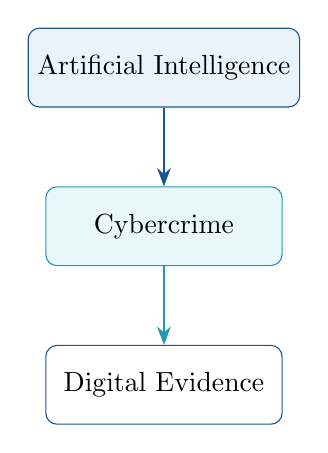
\begin{tikzpicture}[scale=0.8]
				
				\node[
				draw=CyberBlue,
				fill=SoftBlue,
				rounded corners,
				minimum width=3cm,
				minimum height=1cm
				] (AI) {Artificial Intelligence};
				
				\node[
				draw=CyberCyan,
				fill=SoftCyan,
				rounded corners,
				below=1cm of AI,
				minimum width=3cm,
				minimum height=1cm
				] (Attack) {Cybercrime};
				
				\node[
				draw=CyberBlue,
				fill=white,
				rounded corners,
				below=1cm of Attack,
				minimum width=3cm,
				minimum height=1cm
				] (Evidence) {Digital Evidence};
				
				\draw[
				-{Stealth},
				thick,
				CyberBlue
				] (AI) -- (Attack);
				
				\draw[
				-{Stealth},
				thick,
				CyberCyan
				] (Attack) -- (Evidence);
				
			\end{tikzpicture}
			
		\end{columns}
		
	\end{frame}
	
	% =========================================================
	% SLIDE 2
	% =========================================================
	
	\begin{frame}{The Forensic Challenge}
		
		\begin{columns}[T]
			
			\column{0.48\textwidth}
			
			\textbf{Traditional digital forensics}
			
			\begin{itemize}
				\item Identify the device
				\item Acquire the evidence
				\item Preserve integrity
				\item Analyse artefacts
				\item Establish attribution
			\end{itemize}
			
			\column{0.48\textwidth}
			
			\textbf{AI-enabled cybercrime}
			
			\begin{itemize}
				\item Synthetic identities
				\item AI-generated content
				\item Automated attacks
				\item Adversarial manipulation
				\item Difficult attribution
			\end{itemize}
			
		\end{columns}
		
		\vspace{0.5cm}
		
		\begin{alertblock}{Research Question}
			How can digital forensic methods reliably identify, preserve,
			analyse and attribute evidence arising from cybercrimes
			committed using artificial intelligence?
		\end{alertblock}
		
	\end{frame}
	
	% =========================================================
	% SECTION
	% =========================================================
	
	\section{Formalising Digital Evidence}
	
	% =========================================================
	% SLIDE 3
	% =========================================================
	
	\begin{frame}{Formalising Digital Evidence}
		
		Let the set of digital evidence be represented by
		
		\[
		E = \{e_1,e_2,\ldots,e_n\}
		\]
		
		where each element represents a digital artefact.
		
		For example:
		
		\[
		E =
		\{
		\text{email},
		\text{metadata},
		\text{log},
		\text{image},
		\text{network packet}
		\}
		\]
		
		\vspace{0.4cm}
		
		We can define a forensic evidence function:
		
		\[
		F(e_i)=
		\{
		A_i,I_i,P_i,T_i
		\}
		\]
		
		where:
		
		\begin{itemize}
			\item $A_i$ = authenticity
			\item $I_i$ = integrity
			\item $P_i$ = provenance
			\item $T_i$ = temporal information
		\end{itemize}
		
	\end{frame}
	
	% =========================================================
	% SLIDE 4
	% =========================================================
	
	\begin{frame}{Evidence Relationships}
		
		Digital evidence does not exist in isolation.
		
		Consider:
		
		\[
		G=(V,E)
		\]
		
		where:
		
		\begin{itemize}
			\item $V$ represents digital entities;
			\item $E$ represents relationships between entities.
		\end{itemize}
		
		\vspace{0.3cm}
		
		Examples of nodes:
		
		\[
		V=
		\{
		\text{user},
		\text{device},
		\text{account},
		\text{IP},
		\text{email}
		\}
		\]
		
		\vspace{0.2cm}
		
		Examples of edges:
		
		\[
		E=
		\{
		\text{login},
		\text{communication},
		\text{transfer},
		\text{execution}
		\}
		\]
		
		\begin{block}{Forensic implication}
			Graph-based reasoning can help establish relationships between
			apparently independent digital artefacts.
		\end{block}
		
	\end{frame}
	
	% =========================================================
	% SECTION
	% =========================================================
	
	\section{Forensic Framework}
	
	% =========================================================
	% SLIDE 5
	% =========================================================
	
	\begin{frame}{Digital Forensic Evidence Pipeline}
		
		\begin{center}
			
			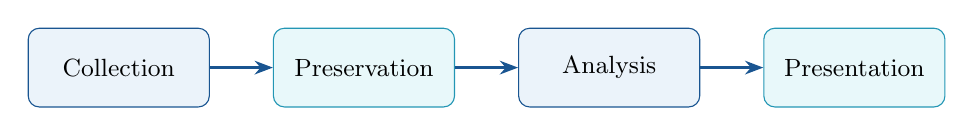
\begin{tikzpicture}[
				node distance=0.8cm,
				every node/.style={
					font=\small
				}
				]
				
				\node[
				draw=CyberBlue,
				fill=SoftBlue,
				rounded corners,
				minimum width=2.3cm,
				minimum height=1cm
				] (C) {Collection};
				
				\node[
				draw=CyberCyan,
				fill=SoftCyan,
				rounded corners,
				minimum width=2.3cm,
				minimum height=1cm,
				right=of C
				] (P) {Preservation};
				
				\node[
				draw=CyberBlue,
				fill=SoftBlue,
				rounded corners,
				minimum width=2.3cm,
				minimum height=1cm,
				right=of P
				] (A) {Analysis};
				
				\node[
				draw=CyberCyan,
				fill=SoftCyan,
				rounded corners,
				minimum width=2.3cm,
				minimum height=1cm,
				right=of A
				] (R) {Presentation};
				
				\draw[
				-{Stealth},
				thick,
				CyberBlue
				] (C) -- (P);
				
				\draw[
				-{Stealth},
				thick,
				CyberBlue
				] (P) -- (A);
				
				\draw[
				-{Stealth},
				thick,
				CyberBlue
				] (A) -- (R);
				
			\end{tikzpicture}
			
		\end{center}
		
		\vspace{0.5cm}
		
		\begin{enumerate}
			\item \textbf{Collection} --- acquire relevant digital artefacts.
			\item \textbf{Preservation} --- protect integrity and provenance.
			\item \textbf{Analysis} --- reconstruct events and relationships.
			\item \textbf{Presentation} --- communicate findings for decision-making.
		\end{enumerate}
		
	\end{frame}
	
	% =========================================================
	% SLIDE 6
	% =========================================================
	
	\begin{frame}{Research Objectives}
		
		\begin{enumerate}
			
			\item Examine existing digital forensic approaches for
			AI-enabled cybercrime.
			
			\vspace{0.25cm}
			
			\item Identify forensic challenges introduced by
			artificial intelligence.
			
			\vspace{0.25cm}
			
			\item Develop a framework for collection, preservation,
			analysis and presentation of AI-related digital evidence.
			
			\vspace{0.25cm}
			
			\item Investigate methods for authenticity, provenance
			and attribution.
			
			\vspace{0.25cm}
			
			\item Validate the proposed framework using appropriate
			forensic scenarios and datasets.
			
		\end{enumerate}
		
	\end{frame}
	
	% =========================================================
	% SECTION
	% =========================================================
	
	\section{Expected Contribution}
	
	% =========================================================
	% SLIDE 7
	% =========================================================
	
	\begin{frame}{Expected Contribution}
		
		\begin{columns}[T]
			
			\column{0.32\textwidth}
			
			\begin{block}{Theoretical}
				Formalisation of forensic reasoning for
				AI-enabled cybercrime.
			\end{block}
			
			\column{0.32\textwidth}
			
			\begin{block}{Technical}
				Methods for analysing authenticity,
				provenance and attribution.
			\end{block}
			
			\column{0.32\textwidth}
			
			\begin{block}{Practical}
				A forensic framework applicable to
				real-world investigations.
			\end{block}
			
		\end{columns}
		
		\vspace{0.7cm}
		
		\begin{center}
			
			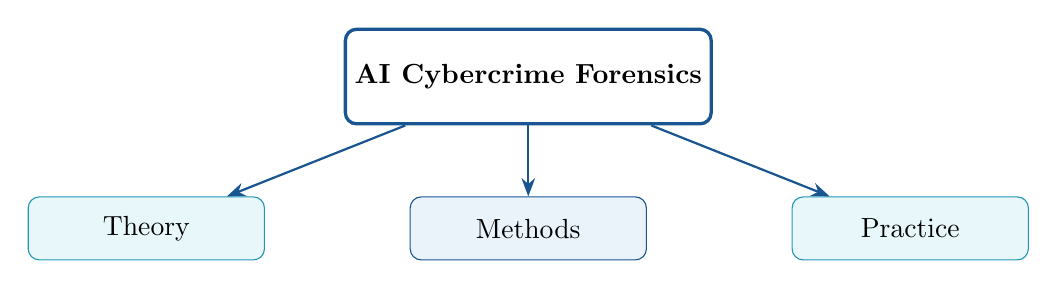
\begin{tikzpicture}
				
				\node[
				draw=CyberBlue,
				fill=white,
				very thick,
				rounded corners,
				minimum width=4cm,
				minimum height=1.2cm
				] (F) {\textbf{AI Cybercrime Forensics}};
				
				\node[
				draw=CyberCyan,
				fill=SoftCyan,
				rounded corners,
				below left=0.9cm and 1cm of F,
				minimum width=3cm,
				minimum height=0.8cm
				] (T) {Theory};
				
				\node[
				draw=CyberBlue,
				fill=SoftBlue,
				rounded corners,
				below=0.9cm of F,
				minimum width=3cm,
				minimum height=0.8cm
				] (M) {Methods};
				
				\node[
				draw=CyberCyan,
				fill=SoftCyan,
				rounded corners,
				below right=0.9cm and 1cm of F,
				minimum width=3cm,
				minimum height=0.8cm
				] (P) {Practice};
				
				\draw[
				-{Stealth},
				thick,
				CyberBlue
				] (F) -- (T);
				
				\draw[
				-{Stealth},
				thick,
				CyberBlue
				] (F) -- (M);
				
				\draw[
				-{Stealth},
				thick,
				CyberBlue
				] (F) -- (P);
				
			\end{tikzpicture}
			
		\end{center}
		
	\end{frame}
	
	% =========================================================
	% SLIDE 8
	% =========================================================
	
	\begin{frame}{Why This Matters}
		
		\begin{block}{The central argument}
			As cybercrime evolves from human-operated attacks toward
			AI-assisted and AI-generated attacks, forensic science must
			also evolve.
		\end{block}
		
		\vspace{0.4cm}
		
		\[
		\boxed{
			\text{AI-enabled crime}
			\quad\Longrightarrow\quad
			\text{AI-aware forensic reasoning}
		}
		\]
		
		\vspace{0.5cm}
		
		The research therefore seeks to bridge:
		
		\begin{center}
			
			\textbf{
				Artificial Intelligence
			}
			\quad $\leftrightarrow$ \quad
			\textbf{
				Cybersecurity
			}
			\quad $\leftrightarrow$ \quad
			\textbf{
				Digital Forensics
			}
			
		\end{center}
		
	\end{frame}
	
	% =========================================================
	% SECTION
	% =========================================================
	
	\section{Conclusion}
	
	% =========================================================
	% SLIDE 9
	% =========================================================
	
	\begin{frame}{Conclusion}
		
		\begin{itemize}
			
			\item AI is changing the nature and scale of cybercrime.
			
			\vspace{0.25cm}
			
			\item Digital evidence associated with AI-enabled crime
			requires stronger methods of authentication and attribution.
			
			\vspace{0.25cm}
			
			\item Formal reasoning, graph analysis and forensic
			methodologies can complement conventional investigations.
			
			\vspace{0.25cm}
			
			\item The proposed research aims to develop a defensible
			framework for AI-enabled cybercrime forensics.
			
		\end{itemize}
		
		\vspace{0.5cm}
		
		\begin{center}
			
			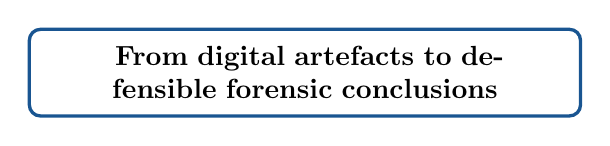
\begin{tikzpicture}
				
				\draw[
				CyberBlue,
				very thick,
				rounded corners
				]
				(0,0) rectangle (7,1.1);
				
				\node[
				align=center,
				text width=6.5cm
				]
				at (3.5,0.55)
				{
					\textbf{
						From digital artefacts to defensible forensic conclusions
					}
				};
				
			\end{tikzpicture}
			
		\end{center}
		
	\end{frame}
	
	% =========================================================
	% THANK YOU
	% =========================================================
	
	\begin{frame}
		
		\begin{center}
			
			\vspace{1cm}
			
			{\Huge\bfseries Thank You}
			
			\vspace{0.5cm}
			
			{\Large Questions and Discussion}
			
			\vspace{1cm}
			
			{\large
				Peter M. Ngugi
			}
			
			\vspace{0.2cm}
			
			{\normalsize
				PhD Computer Science\\
				Zetech University
			}
			
			\vspace{0.8cm}
			
			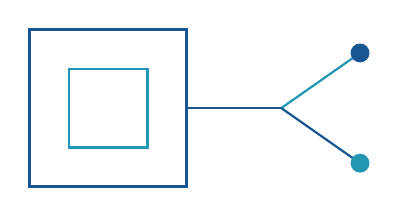
\begin{tikzpicture}
				
				% Technical square
				\draw[
				CyberBlue,
				very thick
				]
				(0,0) rectangle (2,2);
				
				\draw[
				CyberCyan,
				thick
				]
				(0.5,0.5) rectangle (1.5,1.5);
				
				% Connections
				\draw[
				CyberBlue,
				thick
				]
				(2,1) -- (3.2,1);
				
				\draw[
				CyberCyan,
				thick
				]
				(3.2,1) -- (4.2,1.7);
				
				\draw[
				CyberBlue,
				thick
				]
				(3.2,1) -- (4.2,0.3);
				
				% Nodes
				\fill[CyberBlue]
				(4.2,1.7) circle (0.12);
				
				\fill[CyberCyan]
				(4.2,0.3) circle (0.12);
				
			\end{tikzpicture}
			
		\end{center}
		
	\end{frame}
	
	% =========================================================
	% END
	% =========================================================
	
\end{document}